\section{Uruchomienie programu}

Do uruchomienia aplikacji niezbędne jest zainstalowanie biblioteki \emph{MPICH} na każdym komputerze będącym elementem klastra. Prawidłowe działanie programu (w przypadku, w którym chcemy, aby działał on na kilku maszynach) wymaga skonfigurowania połączenia \emph{ssh} , ponieważ ta implementacja standardu \emph{MPI} korzysta z niego jako ze sposobu komunikacji. Zarówno bibliotekę jak i instrukcje konfiguracji można znaleźć na stronie producenta \cite{mpich}. Program uruchamia się z linii komend w następujący sposób:
\begin{center}
\begin{lstlisting}[language=bash, deletekeywords={test}, keepspaces=true, columns=flexible]
mpiexec [-n liczba procesów] -H [adresy komputerów w klastrze oddzielone przecinkami]
./ParallelRayTracing [-s] [-b] [-f nazwa pliku wejściowego] [-w szer. w pikselach]
[-h wys. w pikselach] [-c liczba fragmentów] [-d głębokość drzewa] [-t liczba testów]
\end{lstlisting}
\end{center}
Komenda \emph{mpiexec} jest zdefiniowana w standardzie \emph{MPI} i posiada ona znacznie więcej argumentów opcjonalnych - te wymienione stanowią niezbędne minimum. Liczba procesów musi być ustawiona na więcej niż jeden. Opcja \emph{-H} nie jest konieczna w przypadku uruchamiania aplikacji na jednym komputerze. Jako ostatni parametr komendy \emph{mpiexec} podaje się nazwę programu do uruchomienia wraz z jego parametrami, które zostały niżej omówione.

\begin{itemize}

\item \textbf{-s} - obecność tej flagi włącza śledzenie promieni od punktów przecięcia do źródeł światła - odpowiada ze efekt cieni,
\item \textbf{-b} - obecność tej flagi sprawia, że algorytm korzysta z drzewa BSP,
\item \textbf{-f} - po tej fladze należy podać nazwę pliku z definicją sceny (sposób opisu został podany niżej). Jeżeli nie zostanie ona zdefiniowana program domyślnie szuka pliku ,,scene.txt'',
\item \textbf{-w} - szerokość generowanego obrazu w pikselach. Domyślną wartością jest 700,
\item \textbf{-h} - wysokość generowanego obrazu w pikselach. Domyślną wartością jest 500,
\item \textbf{-c} - liczba fragmentów (zadań) podniesiona do kwadratu, na które zostanie podzielony obraz,
\item \textbf{-d} - głębokość drzewa śledzenia promieni. Domyślna wartość to 3,
\item \textbf{-t} - liczba testów jakie mają wykonać się w ramach uruchomienia programu. Domyślna wartość to 0 - w takiej sytuacji program będzie dział bez końca i nie zwróci wyników działania na konsolę. Jeżeli parametr zostanie ustawiony na wyższą wartość to program zakończy swoje działanie po wygenerowaniu zadanej liczby klatek - czas odpowiedzi danego węzła, jak i czas generowania klatki zostanie uśredniony.

\end{itemize}

%\caption{Przykładowe uruchomienie programu}
\begin{lstlisting}[language=bash]
mpiexec -n 5 ./ParallelRayTracing -s -f spheres.txt -w 640 -h 360
\end{lstlisting}.

Po uruchomieniu programu na ekranie pojawi się okno widoczne na obrazie (!numer obrazka!). W centralnej części interfejsu widzimy podgląd generowanej animacji - obraz obraca się według punktu zdefiniowanego w pliku wejściowym co każdą klatkę animacji (opis pliku wejściowego znajduje się niżej). W dolnej części ekranu widzimy podstawowe informacje związane z czasem generowania obrazu: \emph{SPF} (ang. \emph{second per frame} - czas generowania klatki) i \emph{FPS} (ang. \emph{frames per seconds} - liczba klatek na sekundę). W górnej części interfejsu znajduje klawisz, który otwiera okno z dodatkowymi statystykami (!numer obrazka!). Tabela widoczna w lewej części dodatkowego interfejsu przedstawia średni czas, jaki danemu węzłowi zajmuje liczenie zadania (generowanie fragmentu obrazu). Czas podawany jest w sekundach. W przykładzie pokazanym na obrazku wszystkie procesy liczące znajdują się na komputerze \emph{master}. W prawej części okna podano dodatkowe parametry związane ze sceną.

\begin{figure}[htb!]
\centering
  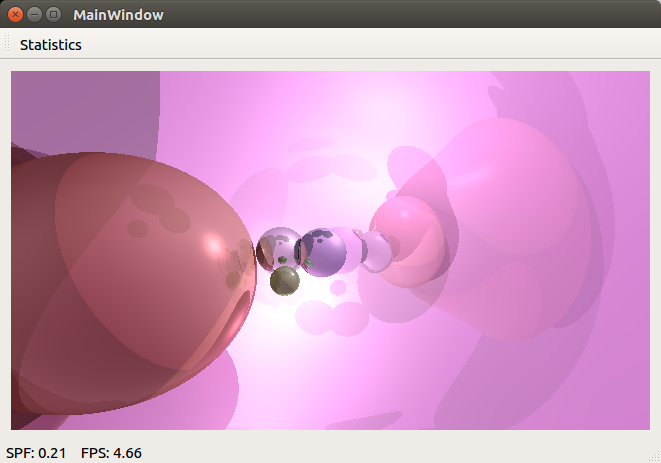
\includegraphics[width=\textwidth]{gui1.png}
  \caption{GUI}
\end{figure}

\begin{figure}[htb!]
\centering
  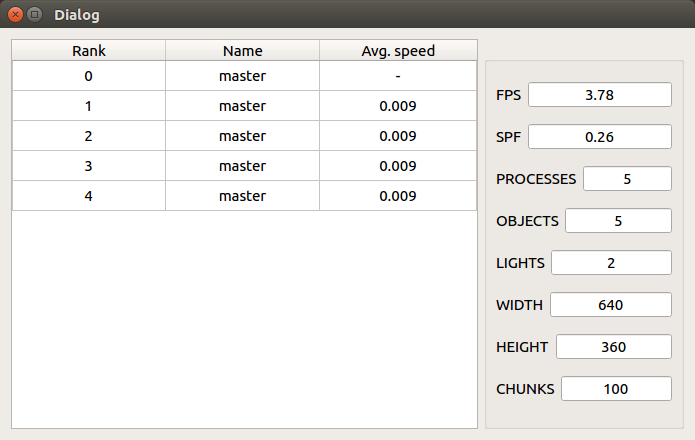
\includegraphics[width=\textwidth]{gui2.png}
    \caption{GUI}
\end{figure}

\section{Opis pliku wejściowego}

Plik wejściowy składa się z szeregu linii definiujących zadane obiekty. Dwa z nich są obowiązkowe i mogą wystąpić w pliku tylko raz (w przypadku podania więcej niż jednej definicji program skorzysta z ostatniej) - \emph{Scene} i \emph{Camera}. Niżej opisano jakie typu obiektów użytkownik może definiować oraz podano przykładowy plik wejściowy. Jeżeli pierwsze słowo w linii (słowo kluczowe) nie zostanie rozpoznane to zostanie on zignorowana. Jeżeli w którymś z parametrów znajduje się błąd obiekt również nie będzie wczytany, ale użytkownik dostanie informację zwrotną o tym, w którym miejscu w pliku pojawił się problem. Parametry są podawane wg. słów kluczowych - ich wartości zawierają się w nawiasach trójkątnych. Jeśli definiowany parametr jest wektorem, kolejne wartości zostają oddzielone przecinkami.

\begin{itemize}

\item \emph{scene} - zawiera parametry światła globalnego i kolor tła.
	\begin{enumerate}
		\item \emph{background} - wektor definiujący kolor tła podany w modelu \emph{RGB}. Wartości powinny zawierać się w przedziale od 0 do 1,
		\item \emph{global} -  wektor określający natężenie światła globalnego (patrz rozdział (RODZIAŁ), \emph{Model Phonga}. Wartości powinny zawierać się w przedziale od 0 do 1,
	\end{enumerate}
	
\item \emph{camera} - definiuje kamerę (obserwatora).

	\begin{enumerate}
		\item \emph{eye} - wektor określający pozycję kamery (oka obserwatora),
		\item \emph{lookAt} - wektor określający punkt, na który patrzy obserwator (to wokół niego będzie się on obracał),
		\item \emph{zNear} - wartość skalarna określająca odległość obserwatora od rzutni (patrz (!rozdział!)
		\item \emph{zFar} -	wartość skalarna określająca maksymalną odległość, na jaką widzi obserwator (patrz (!ROZDZIAŁ!)
		\item \emph{povy} -	wartość skalarna określająca pionowy kąt widzenia obserwatora (patrz (!ROZDZIAŁ!). Jest ona podawana w stopniach.
	\end{enumerate}

\item \emph{light} - definiuje właściwości i położenie punktowego źródła światła

	\begin{enumerate}
		\item \emph{pos} - wektor określający pozycję światła.
		\item \emph{amb} - wektor określający, w jaki sposób źródło światła wpływa na oświetlenie otoczenia (ang. \emph{ambient light} - patrz (!ROZDZIAŁ!))
		\item \emph{dif} - wektor określający natężenie światła rozproszonego (ang. \emph{diffuse light} - patrz (!ROZDZIAŁ!))
		\item \emph{spec} - wektor określający natężenie światła kierunkowego (ang. \emph{specular light} - patrz (!ROZDZIAŁ!))
	\end{enumerate}

\item \emph{triangle}

	\begin{enumerate}
		\item \emph{pointA} - wektor określający położenie jednego z wierzchołków trójkąta.
		\item \emph{pointB} - wektor określający położenie jednego z wierzchołków trójkąta.
		\item \emph{pointC} - wektor określający położenie jednego z wierzchołków trójkąta.
		\item \emph{amb} - wektor określający procentowy wpływ światła otoczenia na powierzchnię (ang. \emph{ambient light} - patrz (!ROZDZIAŁ!)). Wartości powinny zawierać się w przedziale od 0 do 1,
		\item \emph{dif} - wektor określający procentowy wpływ światła rozproszonego na powierzchnię (ang. \emph{diffuse light} - patrz (!ROZDZIAŁ!). Wartości powinny zawierać się w przedziale od 0 do 1,
		\item \emph{spec} - wektor określający procentowy wpływ światła kierunkowego na powierzchnię (ang. \emph{specular light} - patrz (!ROZDZIAŁ!)). Wartości powinny zawierać się w przedziale od 0 do 1,
		\item \emph{specShin} - skalar, który wpływa na wygląd odblasków na powierzchni (przyjmuje wartości od kliku do kilkuset).
		\item \emph{trans} - skalar określający procentowy wpływ przezroczystości przedmiotu na kolor powierzchni (w przypadku zera nie jest wysyłany promień przechodzący przez powierzchnię). Wartości zawierać się w przedziale od 0 do 1,
		\item \emph{mirror} - skalar określający procentowy wpływ promieni odbitych na ostateczny kolor piksela (w przypadku zera nie jest wysyłany żaden promień odbity).
		\item \emph{local} - parametr skalarny określający procentowy wpływ właściwych parametrów powierzchni na kolor piksela.
		\item \emph{density} - skalar określający gęstość przedmiotu (współczynniki gęstości są stabelaryzowane i dostępne w Internecie), która wpływa na złamanie światła. Gęstość ośrodka sceny wynosi 1.
	\end{enumerate}

\item \emph{sphere}

	\begin{enumerate}
		\item \emph{amb} - wektor określający procentowy wpływ światła otoczenia na powierzchnię (ang. \emph{ambient light} - patrz (!ROZDZIAŁ!)). Wartości powinny zawierać się w przedziale od 0 do 1,
		\item \emph{dif} - wektor określający procentowy wpływ światła rozproszonego na powierzchnię (ang. \emph{diffuse light} - patrz (!ROZDZIAŁ!). Wartości powinny zawierać się w przedziale od 0 do 1,
		\item \emph{spec} - wektor określający procentowy wpływ światła kierunkowego na powierzchnię (ang. \emph{specular light} - patrz (!ROZDZIAŁ!)). Wartości powinny zawierać się w przedziale od 0 do 1,
		\item \emph{specShin} - skalar, który wpływa na wygląd odblasków na powierzchni (przyjmuje wartości od kliku do kilkuset).
		\item \emph{trans} - skalar określający procentowy wpływ przezroczystości przedmiotu na kolor powierzchni (w przypadku zera nie jest wysyłany promień przechodzący przez powierzchnię).
		\item \emph{pos} - wektor określający położenie środka sfery.
		\item \emph{radius} - skalar określający promień sfery.
		\item \emph{trans} - skalar określający procentowy wpływ przezroczystości przedmiotu na kolor powierzchni (w przypadku zera nie jest wysyłany promień przechodzący przez powierzchnię). Wartości zawierać się w przedziale od 0 do 1,
		\item \emph{mirror} - skalar określający procentowy wpływ promieni odbitych na ostateczny kolor piksela (w przypadku zera nie jest wysyłany żaden promień odbity).
		\item \emph{local} - parametr skalarny określający procentowy wpływ właściwych parametrów powierzchni na kolor piksela.
		\item \emph{density} - skalar określający gęstość przedmiotu (współczynniki gęstości są stabelaryzowane i dostępne w Internecie), która wpływa na złamanie światła. Gęstość ośrodka sceny wynosi 1.
	\end{enumerate}

\item \emph{obj} - po tym słowie kluczowym należy podać nazwę pliku \emph{obj} (wraz z rozszerzeniem). Program wczyta ten plik konwertując wielokąty w nim zdefiniowane na trójkąty. Pliki \emph{.obj} mogą wskazywać na pliki \emph{.mtl} zawierające definicję materiałów z nimi związanych. Jeżeli taki plik znajduje się w katalogu z programem, to również zostanie on wczytany. W przeciwnym wypadku zostanie zastosowany materiał domyślny.

\lstinputlisting[language={}]{exampleinput.txt}


\end{itemize}
